%-- coding: UTF-8 --
%
\documentclass{llncs}
\usepackage{amsfonts}
\usepackage{amstext}
\usepackage{amsmath}
\usepackage{enumitem}
\usepackage{multirow}
\usepackage{graphicx}
\usepackage[center]{subfigure}
\usepackage{amssymb}
\usepackage{graphicx,amsmath}
\usepackage{subfigure}
\usepackage{algorithm}
\usepackage{algorithmic}
\renewcommand{\algorithmicrequire}{ \textbf{Input:}}
\renewcommand{\algorithmicensure}{ \textbf{Output:}}
\usepackage{url}
\usepackage{cite}
\usepackage{color}
\usepackage[UTF8]{ctex}
%
\begin{document}

\title{知识表示学习模型的研究}
\author{Anonymous}
\institute{北京航空航天大学计算机学院}
\maketitle

\begin{abstract}

摘要。

\keywords{表示学习,知识图谱,知识表示}

\end{abstract}

\section{引言}

知识图谱是一种可以结构化地表示真实世界中的实体和实体间关系的网络,广泛应用于搜索引擎等领域。近年来,大量开源知识图谱,如 WordNet\cite{Miller:1995:WLD:219717.219748} 、 Freebase\cite{Bollacker:2008:FCC:1376616.1376746} 和 Yago\cite{suchanek2007yago} 的出现,验证了知识图谱模型在真实世界数据集中的表现。而知识表示学习\cite{DBLP:journals/corr/abs-1812-10901},则是将知识图谱中的实体和关系用词向量的形式来表示,使得知识图谱相关研究不必拘束于图的算法。本文将针对近年来具有重要意义的知识表示学习模型进行研究和对比,并介绍知识表示学习的相关应用。

\section{背景介绍}

\subsection{知识图谱}

知识图谱是用来表示真实世界中的实体和实体间关系的图结构网络,由节点和边组成,其中节点代表实体,边代表实体之间的关系,通常用三元组 $G=\{E,R,S\}$ 来表示知识图谱,其中 $E$ 为实体的集合, $R$ 为关系的集合, $S$ 是实体-关系-实体的三元组集合,即 $S\subseteq{E×R×E}$ 。此外,一个实体-关系-实体的三元组也可以表示为 $(h,r,t)$ 的格式,其中 $h$ 和 $t$ 分别代表头实体和尾实体, $r$ 表示头实体和尾实体之间的关系。

著名知识图谱开源数据集有 WordNet 、 FreeBase 和 Yago 等。其中 WordNet 数据集是由专家构建的词典知识库, FreeBase 数据集则是由志愿者构建的世界知识库,包含人物、地点、分类等信息, Yago 则是一个从半结构化文本中学习出的知识库。知识表示学习的相关算法,大多基于 WordNet 和 FreeBase 进行验证。但在 ConvE 模型\cite{DBLP:conf/aaai/DettmersMS018}中发现,这两个数据集的子集 FB15K 和 WN18 存在严重的测试集泄漏问题,即对于某个训练集中的三元组,反转其头实体和尾实体,就可以在测试集中找到相同的数据。故在此后的研究中,普遍使用去除泄漏数据的 FB15K-237 和 WN18-RR 数据集进行训练、验证和预测。

\subsection{知识表示学习}

知识图谱通常以图的形式存储,这种图结构不仅不利于对知识图谱的进一步研究,更需要设计特定的算法进行相应的计算。因此通常将图结构转化为向量的形式,便于更加高效的解决知识图谱领域的关系提取、关系预测、实体预测等问题。

通过向量表示实体的方法通常有两种。在传统方法中,采用独热编码来构建向量。对一个有n个实体数据集,需要对每个实体使用一个n维向量来表示。每个向量中只有1维的值为1,其余值均为0。这种方法存在明显的问题:随着数据集规模的增加,向量维数过大;又由于向量之间两两正交,不仅无法表示出实体的语义信息,更无法表示实体之间的相似程度。另一种构建词向量的方法则是通过机器学习算法,得到每一个实体的低维稠密向量。对于一个词向量而言,单独拿出一维数值可能毫无意义,但组成词向量后却可以表示出相应实体的语义信息,这就是表示学习。

所谓知识表示学习,即对知识库运用表示学习的方法。通过用低维度的稠密向量来表示知识库中的实体或关系,从而进行实体预测、实体分类、语义相似性分析等工作。常用的知识表示学习模型可以分为线性模型、神经网络模型、翻译模型等。

\section{知识表示学习模型}

\subsection{距离模型及其扩展模型}

结构表示模型(Structured Embeddings,SE)\cite{DBLP:conf/aaai/BordesWCB11}是最经典的线性模型, SE 模型也被称为距离模型。对于知识图谱中的一个头实体-尾实体-关系三元组 $\{E_h, E_t, R_k\}$ , SE 模型通过将第 $x$ 个实体 $E_x$ 表征为一个 $d$ 维(约50维)的词向量 $l_x$ ,将第 $k$ 个关系 $R_k$ 构造成两个 $d×d$ 维的投影矩阵 $W^h_k$ 和 $W^t_k$ ,并定义了如下的损失函数来计算实体之间的语义相关性:
\begin{displaymath}
S_k(E_h,E_t)=||W^h_kl_h-W^t_kl_t||_p
\end{displaymath}
在 SE 模型中,取范数 $p=1$ ,此时损失函数为:
\begin{displaymath}
S_k(E_h,E_t)=\sum_{x=1}^d{S_k(E_h,E_t)_x}
\end{displaymath}
即将头实体和尾实体的词向量分别用一个投影矩阵投影,投影后的距离为投影后得到的向量差按位相加的结果。 SE 模型认为,实体投影后的距离越小,头实体和尾实体的越有可能存在该种关系。因此只需不断迭代使得损失函数最小,求出实体向量 $l$ 和投影矩阵 $W$ 两个参数的最优值。应用在实体预测时,只需通过头实体词向量和两个关系矩阵,即可计算出尾实体映射在该关系空间中的词向量。由于损失函数采用 $L1$ 范数, SE 模型又被称为距离模型。

但使用两个投影矩阵来定义一种关系,很难直观的表征出实体之间的关系。在现实世界中,实体 king 与 queen 之间的关系,应该和实体 man 与 woman 的关系有一定联系。换言之,这两个关系向量应该具有某种相似性。但 SE 模型通过两个投影矩阵来表示一种联系后,很难反映出其中的语义联系。此后出现的单层感知机模型(Single Layer Model,SLM)\cite{DBLP:conf/nips/SocherCMN13}和多层感知机模型(Multi Layer Perceptron,MLP)\cite{DBLP:conf/kdd/0001GHHLMSSZ14},试图在 SE 模型的基础上解决这个问题。 SLM 模型采用了和 SE 模型一样的两个投影矩阵,其评价函数为:
\begin{displaymath}
g(E_h,E_t,R_k)=u_k^Ttanh(W^h_kl_h+W^t_kl_t)
\end{displaymath}
其中 $u_k$ 为关系 $R_k$ 相关的参数。而 MLP 模型可以看作在 SLM 模型的基础上引入多个隐藏层的结果。 SLM 模型和 MLP 模型并非线性模型,而是利用神经网络进行计算,由此带来了挖掘实体和关系之间隐含语义联系的可能性,一定程度上解决了 SE 模型中无法计算实体之间和关系之间的语义联系的问题,但与此同时也大幅提高了参数计算的复杂度。

为了进一步解决距离模型中,使用两个投影矩阵无法直观表现关系之间的语义联系的问题,出现了双线性模型。所谓双线性,即头实体向量 $l_h$ 或尾实体向量 $l_t$ 都可以通过一个关系矩阵的线性变换得到对方。隐变量模型(Latent Factor Model,LFM)\cite{DBLP:conf/nips/JenattonRBO12}和DistMult模型\cite{DBLP:journals/corr/YangYHGD14a}就是双线性模型的代表。 LFM 模型可以直观的通过其评价函数来理解:
\begin{displaymath}
g(E_h,E_t,R_k)=l_h^TW_kl_t^T
\end{displaymath}

张量神经网络模型(Neural Tensor Networks,NTN)\cite{DBLP:conf/nips/SocherCMN13}则是双线性模型和神经网络模型的结合。

\subsection{翻译模型及其扩展模型}

\subsection{其它模型}

% \begin{figure}
% 	\centering
% 	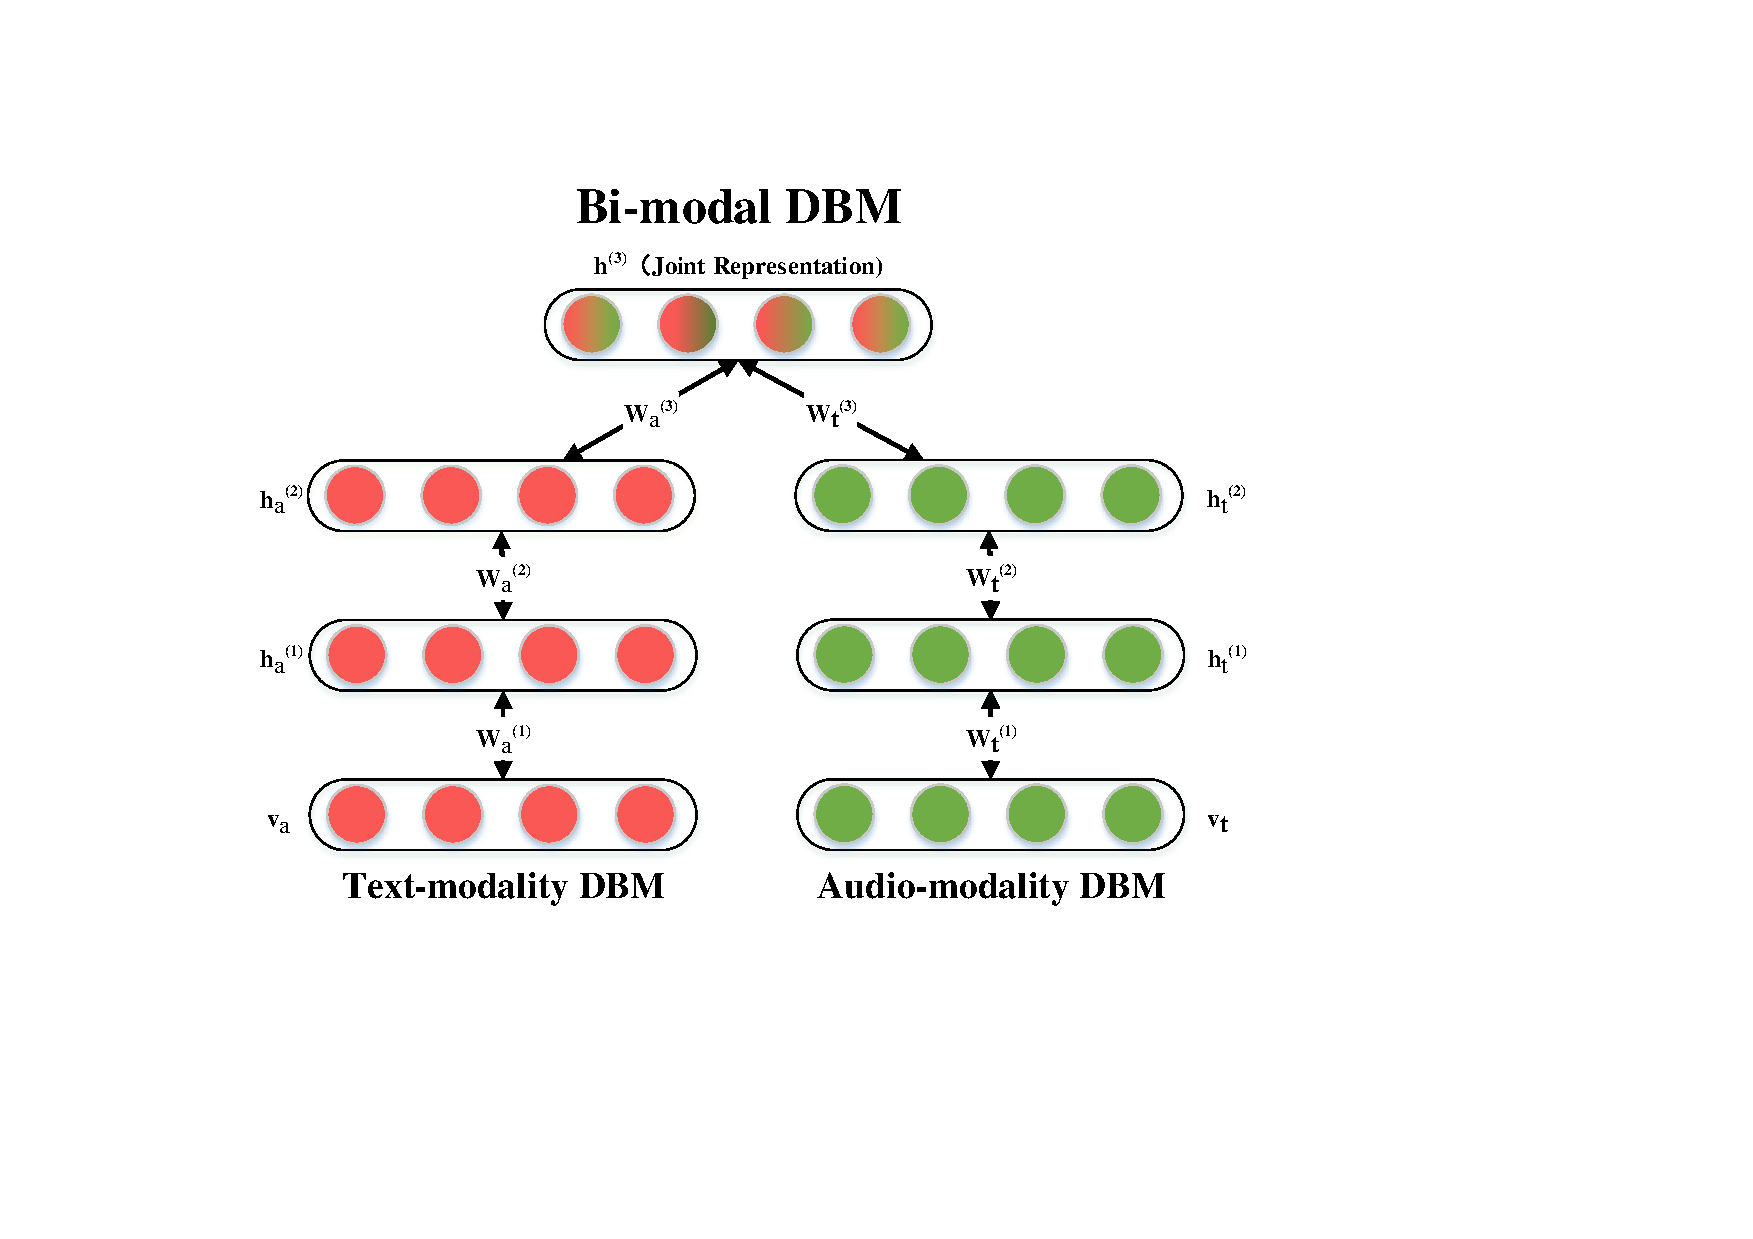
\includegraphics[width=0.5\columnwidth]{figures/bi-modalDBM}
% 	%  \setlength{\abovecaptionskip}{0pt}
% 	%  \setlength{\belowcaptionskip}{-20pt}
% 	\caption{Bi-modal Deep Boltzmann Machine}
% 	\label{fg:DBM}
% \end{figure}

% \begin{table}
% 	\centering
% 	\caption{Mood quadrants and their corresponding number of songs}
% 	\label{tb:clas-scheme}
% 	\begin{tabular}{|c|l|l|c|}
% 		\hline
% 		\textbf{Quadrant}               & \multicolumn{1}{c|}{\textbf{Group}} & \multicolumn{1}{c|}{\textbf{Tag}} & \textbf{Songs}         \\ \hline
% 		\multirow{2}{*}{$v^{-}a^{+}$} & G29                                 & aggressive,aggression.            & \multirow{2}{*}{28,168} \\ \cline{2-3}
% 		& G28                                 & anger,angry,choleric,etc.         &                         \\ \hline
% 		\multirow{2}{*}{$v^{+}a^{+}$} & G6                                  & cheerful,jolly,festive,etc.       & \multirow{2}{*}{16,315} \\ \cline{2-3}
% 		& G5                                  & happy,happiness,etc.              &                         \\ \hline
% 		\multirow{3}{*}{$v^{-}a^{-}$} & G15                                 & sad,sadness,unhappy,etc.          & \multirow{3}{*}{10,154} \\ \cline{2-3}
% 		& G16                                 & depressed,blue,dark,gloom,etc.    &                         \\ \cline{2-3}
% 		& G17                                 & heartbreak,grief,sorrow,etc.      &                         \\ \hline
% 		\multirow{2}{*}{$v^{+}a^{-}$}  & G8                                  & brooding,contemplative,etc.       & \multirow{2}{*}{2,629}  \\ \cline{2-3}
% 		& G12                                 & calm,comfort,quiet,etc.           &                         \\ \hline
% 	\end{tabular}
% \end{table}


\section{结论}% and Future Works}

\subsubsection*{Acknowledgements}

\bibliographystyle{splncs03}
%\bibliographystyle{unsrt}
\bibliography{reference}
	
\end{document}
